% General settings
\documentclass[slidestop,compress,9pt]{beamer}
\usetheme{AnnArbor}
\usepackage[UKenglish]{babel}
\usepackage[UKenglish]{isodate}
\usepackage[utf8]{inputenc}
\usepackage{hyperref}
\definecolor{links}{HTML}{2A1B81}
\hypersetup{colorlinks=true,allcolors=links}

% Code listings and pseudocode
\usepackage{listings}
\usepackage{algpseudocode}
\usepackage{algorithm}

% Mathematical formulas
\usepackage{amsmath}
\usepackage{mathtools}
\usepackage{bm}
\setcounter{MaxMatrixCols}{20}

% Graphics and figures
\usepackage{graphicx}
\graphicspath{{figures/}}
\setbeamertemplate{caption}[numbered]
\usepackage{fancybox}
\usepackage{pgfplots}

% Tikz
\usepackage{tikz}
\usepackage{tikz-3dplot}
\usetikzlibrary{shapes.geometric, arrows}

% For redefinition of texttt
%\let\textttorig\texttt
\usepackage[scaled=1.0]{couriers}

\setbeamertemplate{frametitle}{\thesection.~\insertsection\hspace*{0.45cm}\insertframetitle}

% Numbered sections
\setbeamertemplate{section in toc}[sections numbered]
\setbeamertemplate{subsection in toc}[subsections numbered]
\setbeamertemplate{subsubsection in toc}[subsubsections numbered]

% Listings
\definecolor{cident}{rgb}{0.0,0.0,0.0}
\definecolor{ckeyw}{rgb}{0,0,0.8}
\definecolor{ccomm}{rgb}{0,0.8,0}
\definecolor{cstr}{rgb}{0.8,0,0}
\definecolor{myyellow}{rgb}{0.99,0.76, 0.0}
\definecolor{mymagenta}{rgb}{1.0, 0.0, 1.0}

\lstset{language=Python,
  basicstyle=\small\ttfamily,
  keywordstyle=\color{ckeyw}\bfseries,
  identifierstyle=\color{cident}\bfseries,
  commentstyle=\color{ccomm},
  stringstyle=\color{cstr},
  showstringspaces=false,
  breaklines=true,
  breakatwhitespace=true,
  tabsize=2,
  mathescape = false,
  columns=flexible,
  escapeinside={<@}{@>}
%   numbers=left,
%   stepnumber=1,
%   firstnumber=1,
%   numberfirstline=true,
  }

\title[The oxDNA Coarse-Grained Model of DNA and RNA]{\textbf{The oxDNA Coarse-Grained Model of DNA}}
\subtitle{An Introduction to the Model and Software Framework }
\author[Oliver Henrich]{Oliver Henrich \\ \small Email: \href{mailto:oliver.henrich@strath.ac.uk}{oliver.henrich@strath.ac.uk}}
\institute[U Strathclyde, Glasgow, UK]{Department of Physics, University of Strathclyde, Glasgow, UK}
\date{22nd September 2022}


\begin{document}

%\renewcommand<>{\texttt}[1]{%
%  \only#2{\textttorig{#1}}%
%}

\renewcommand<>{\texttt}{\only#1{\beameroriginal{\texttt}}}

% ==============================================================
% --- Welcome frame
% ==============================================================
\begin{frame}[plain]
\maketitle
\end{frame}

% ==============================================================
% --- TOC
% ==============================================================

\begin{frame}
\Large Outline
\normalsize
\tableofcontents
\end{frame}

% ==============================================================
% --- Content
% ==============================================================

\section{oxDNA Model}

\begin{frame}
\frametitle{DNA Facts}

\begin{itemize}
\item Human genome contains $3\times10^{9}$ base pairs (bps)
\item DNA loop around a nucleosome core particle contains 147 bps
\item Smallest loop in chromatin fibre consists of $5\times10^4$ bps
\item Atomistic simulation of DNA can model 3,000 bps (probably less) and typically resolve times on the $\mu$s-scale  
\item \textbf{Coarse-grained models} target much \textbf{larger time and length scales} in the range of ms and Mbps 
\end{itemize}

\begin{center}
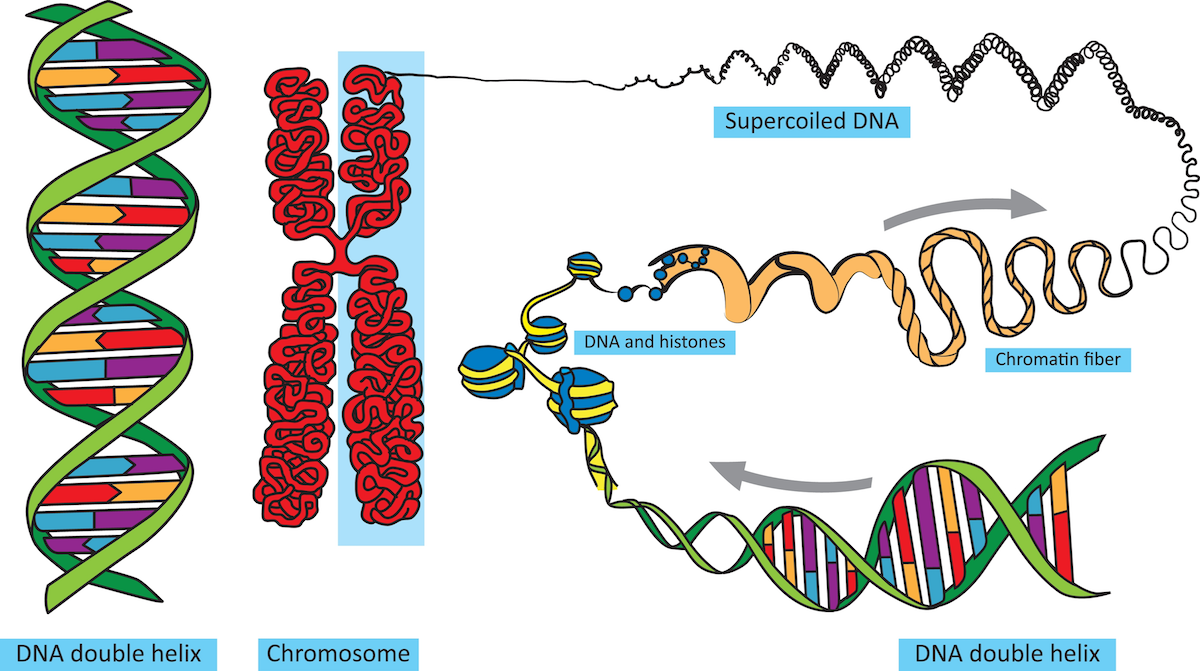
\includegraphics[width=0.54\textwidth]{fromDNAtoChromatin.png}
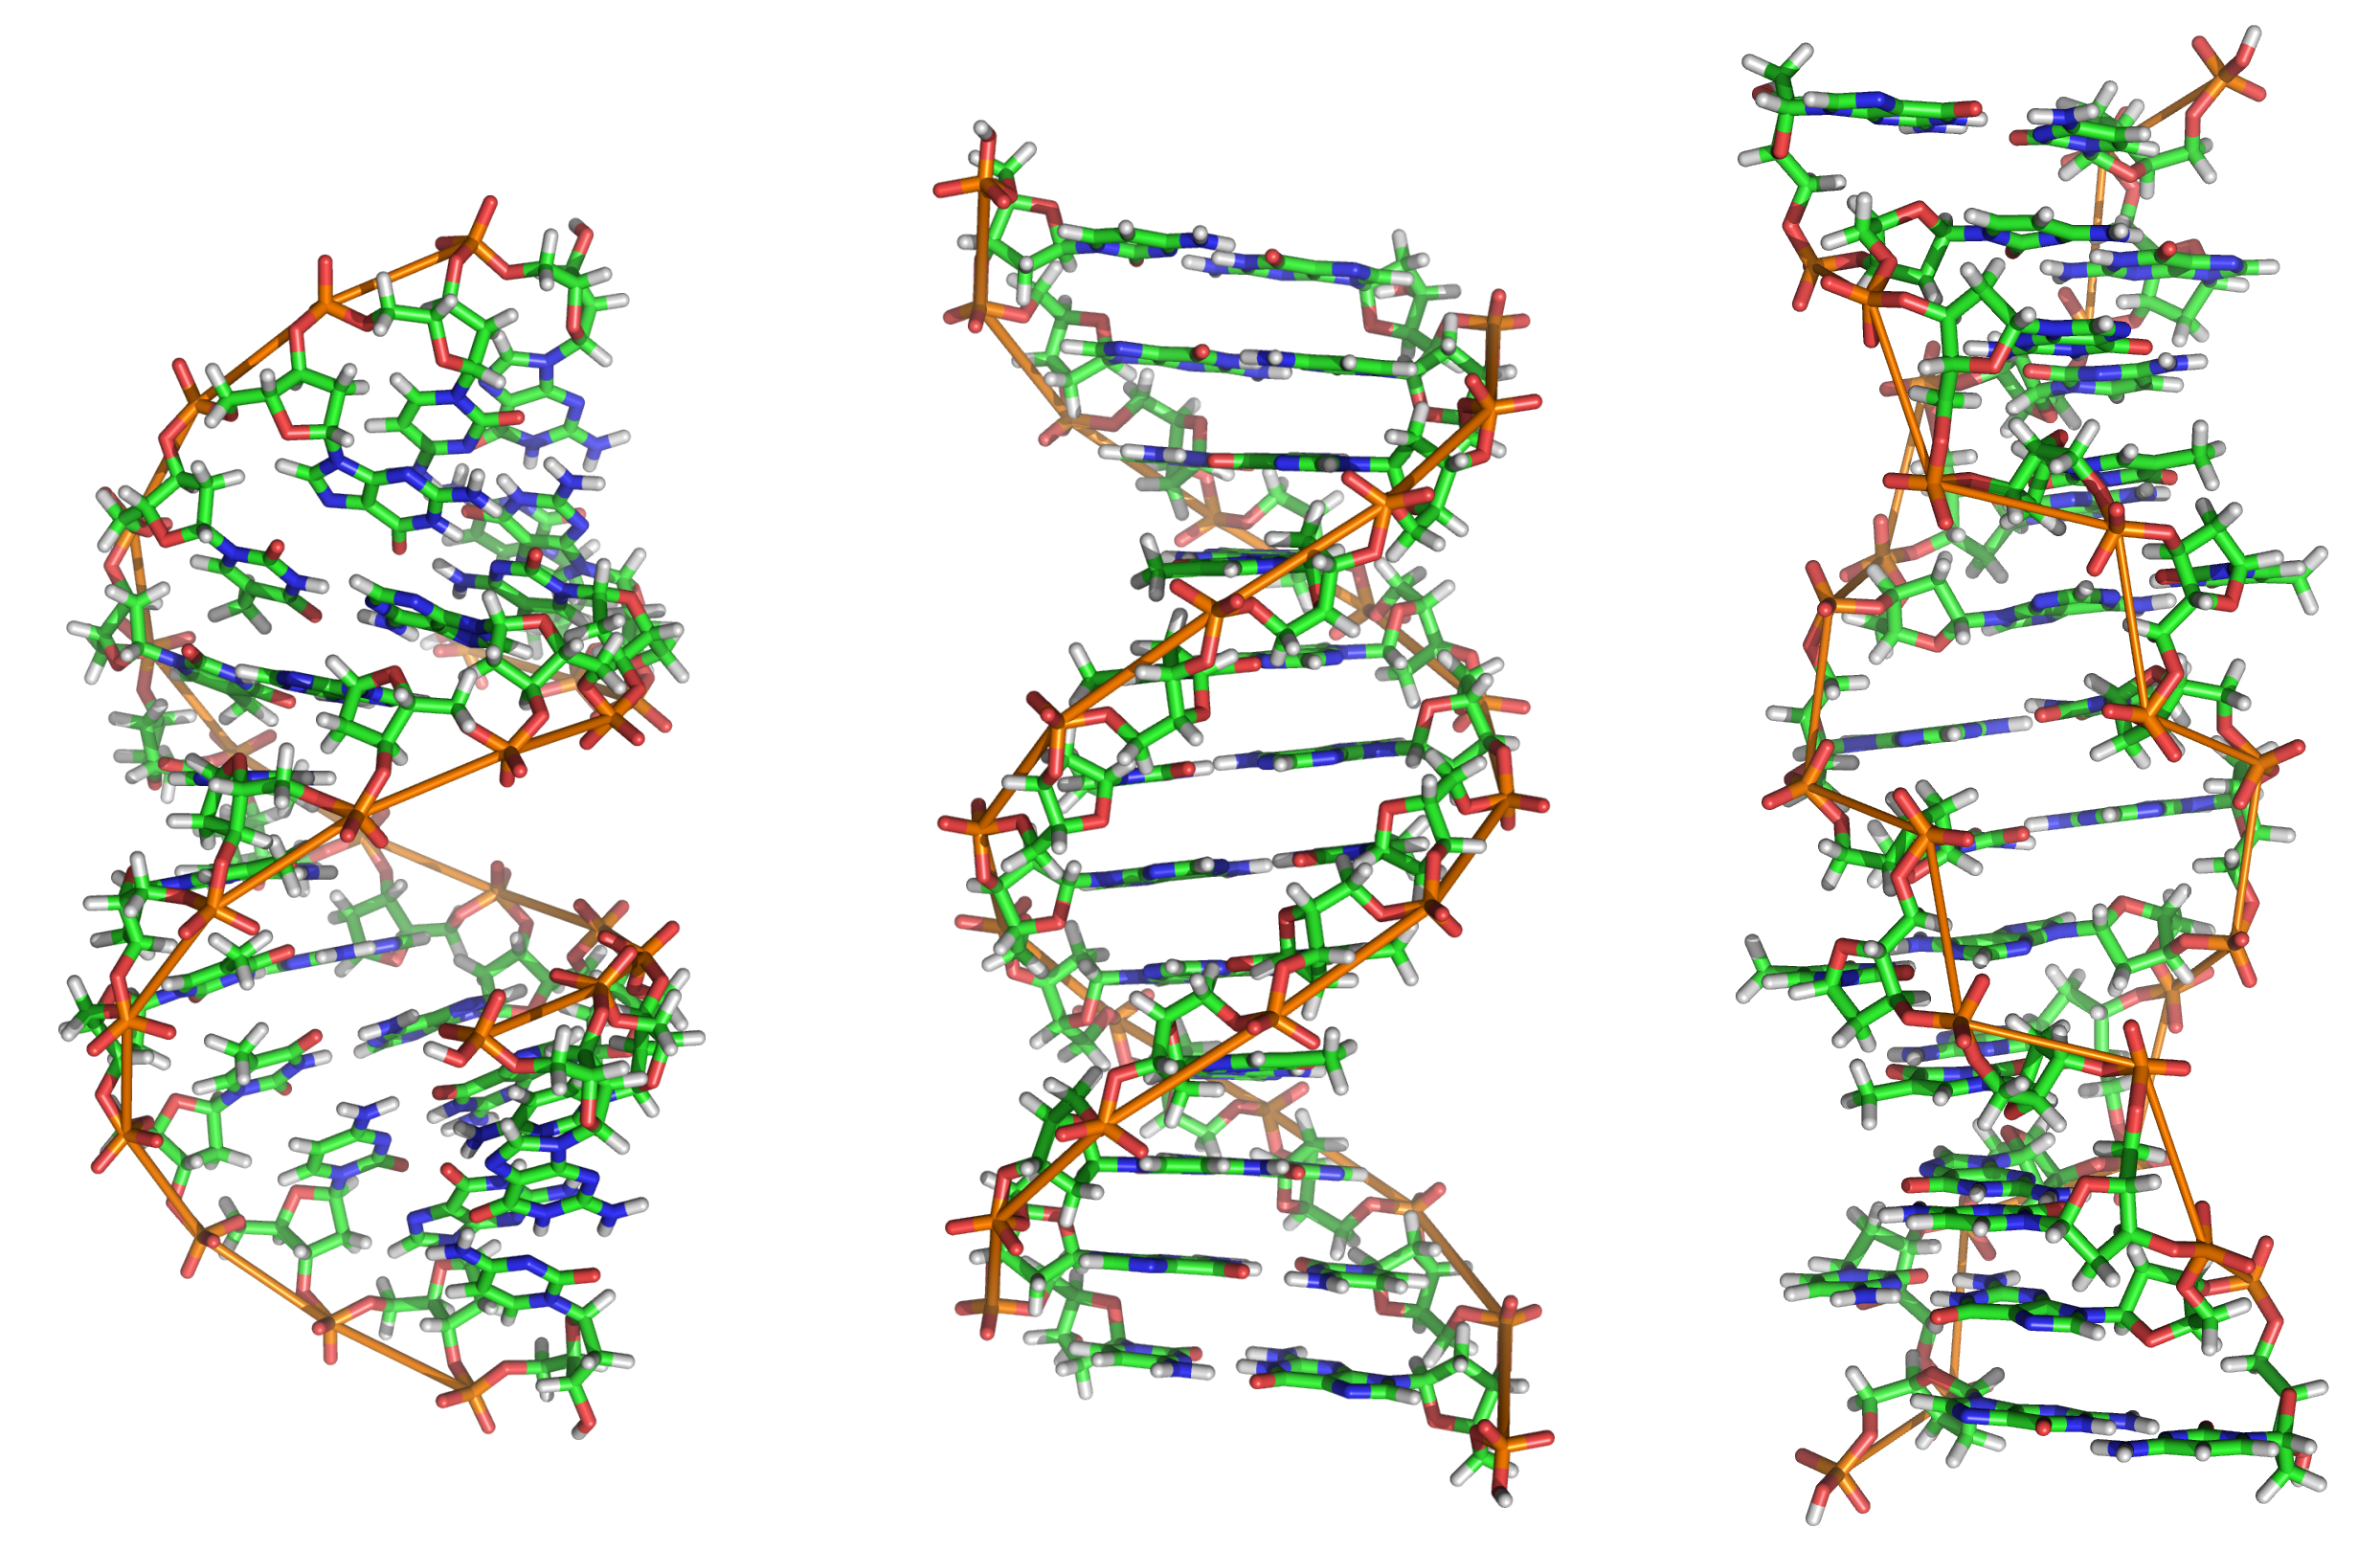
\includegraphics[width=0.45\textwidth]{A-B-Z-DNA.png}\\
\textit{From DNA to chromatin} \hspace{2.75cm} \textit{A-DNA, B-DNA, Z-DNA}
\end{center}

\end{frame}

\begin{frame}
\frametitle{Overview}

\begin{itemize}
\item \textbf{Each nucleotide} is described as \textbf{rigid body}
\item \textbf{3 interaction} sites for backbone, stacking and hydrogen-bonding
\item \textbf{7 effective interactions} between nucleotides
\begin{itemize}
\item Bonded interaction for backbone connectivity
\item 6 pair interactions for excluded volume, stacking, cross-stacking, coaxial stacking, hydrogen-bonding and electrostatic interaction
\end{itemize}
\item \textbf{oxDNA: 13 DOF per nucleotide}\\
3 positions, 3 translational momenta, 3 angular momenta, 1 unit quaternion (4 components)
\item \textbf{Atomistic simulation} (pyrimidine base plus sugar-phosphate group):\\
around \textbf{200 DOF per nucleotide}\\
34 atoms per nucleotide, each with 3 positions and 3 momenta
\end{itemize}

\vspace*{-0.5cm}

\begin{columns}
\begin{column}{0.4\textwidth}
\begin{center}
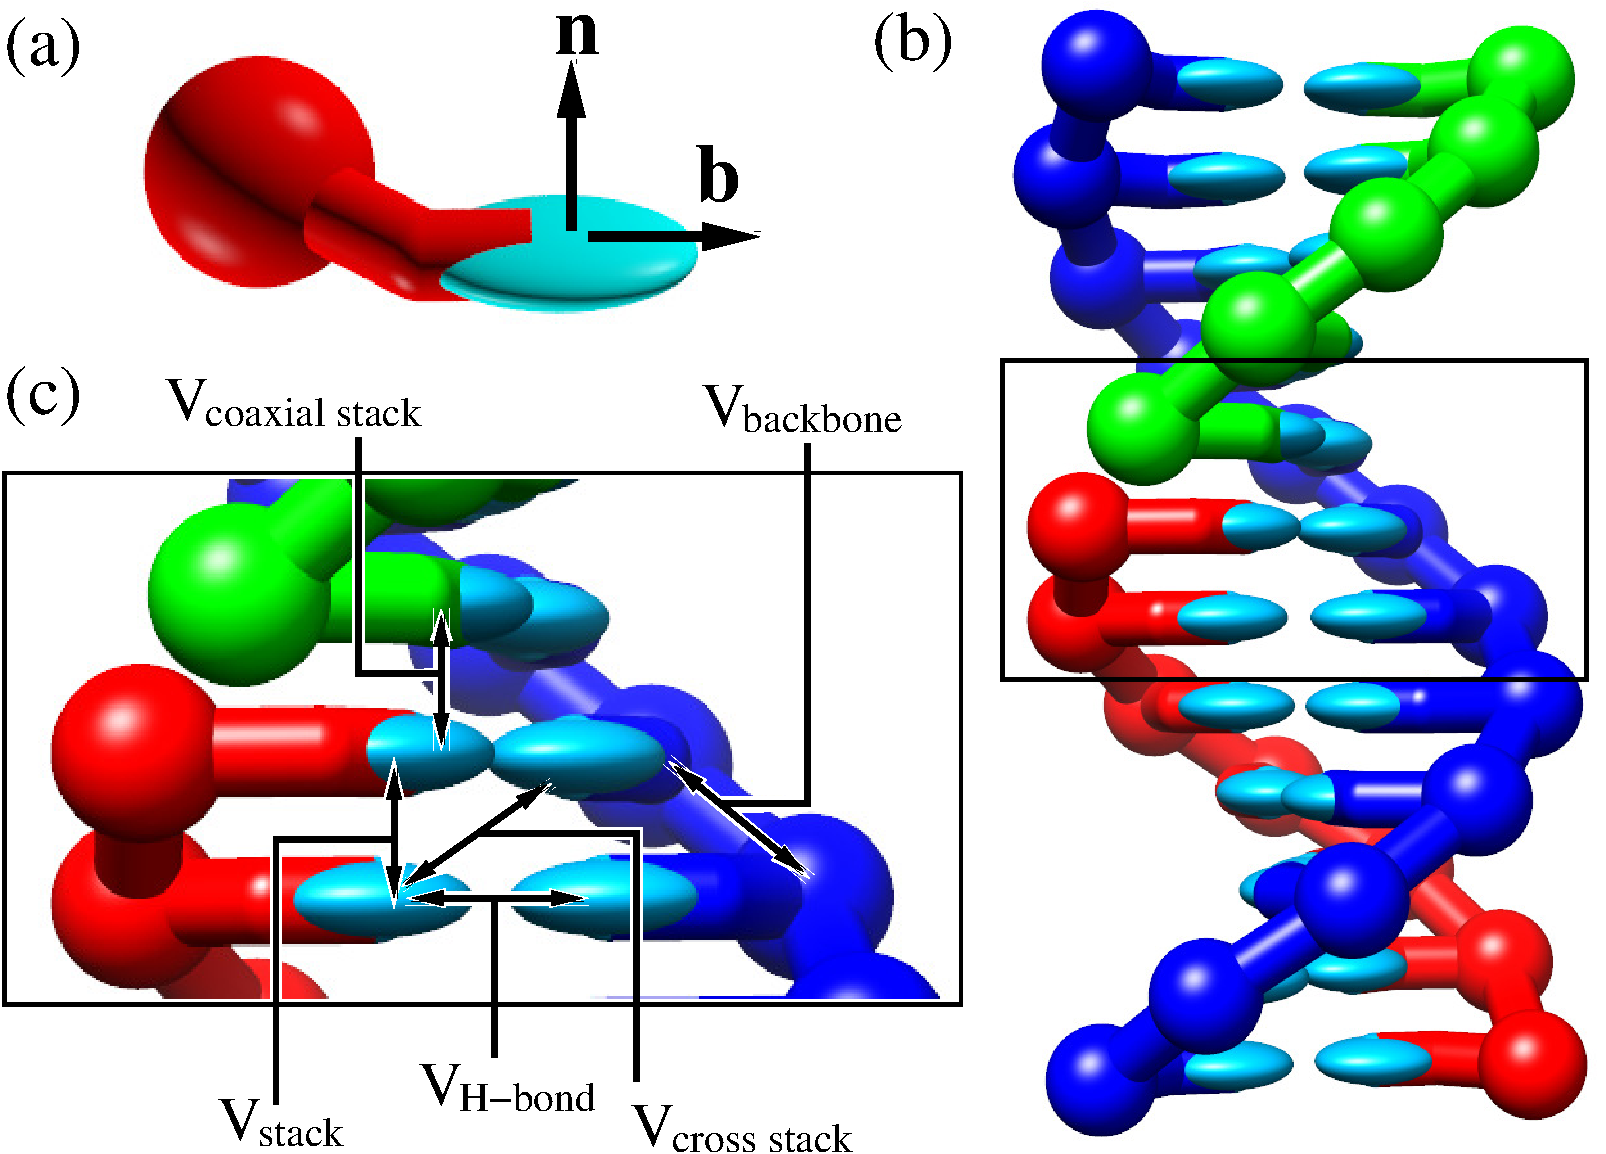
\includegraphics[width=0.9\textwidth]{nucleotide_duplex_b.pdf}
\end{center}
\end{column}

\begin{column}{0.45\textwidth}
\begin{center}
\vspace*{0.5cm}
\begin{itemize}
\setlength\itemsep{7pt}
\item[] \textit{(a) oxDNA nucleotide}
\item[] \textit{(b) Duplex}
\item[] \textit{(c) Interactions}
\end{itemize}
\end{center}
\end{column}
\end{columns}

\end{frame}

\begin{frame}
\frametitle{Nucleotide Geometry}

\begin{columns}
\begin{column}{0.56\textwidth}
\begin{itemize}
\setlength\itemsep{20pt}
\item Each nucleotide has a centre of mass (COM) $\bm{r}_{COM}$, a base vector $\bm{b}$, base normal $\bm{n}$ and a third vector $\bm{y}=\bm{n}\times\bm{b}$
\item The \textbf{backbone interaction} site is at\\
$\bm{r}_{back}=\bm{r}_{COM} - 0.4\,\bm{b}$ \hspace{1.7cm}(oxDNA1)\\
$\bm{r}_{back}=\bm{r}_{COM} - 0.34\, \bm{b} + 0.3408\,\bm{y}$ (oxDNA2)
\item The \textbf{stacking interaction} site is at\\
$\bm{r}_{stack}=\bm{r}_{COM} + 0.34\, \bm{b}$
\item The \textbf{hydrogen-bonding interaction} site is at\\
$\bm{r}_{base}=\bm{r}_{COM} + 0.4\, \bm{b}$
\end{itemize}
\end{column}

\begin{column}{0.44\textwidth}
\vspace*{-0.5cm}
\begin{center}
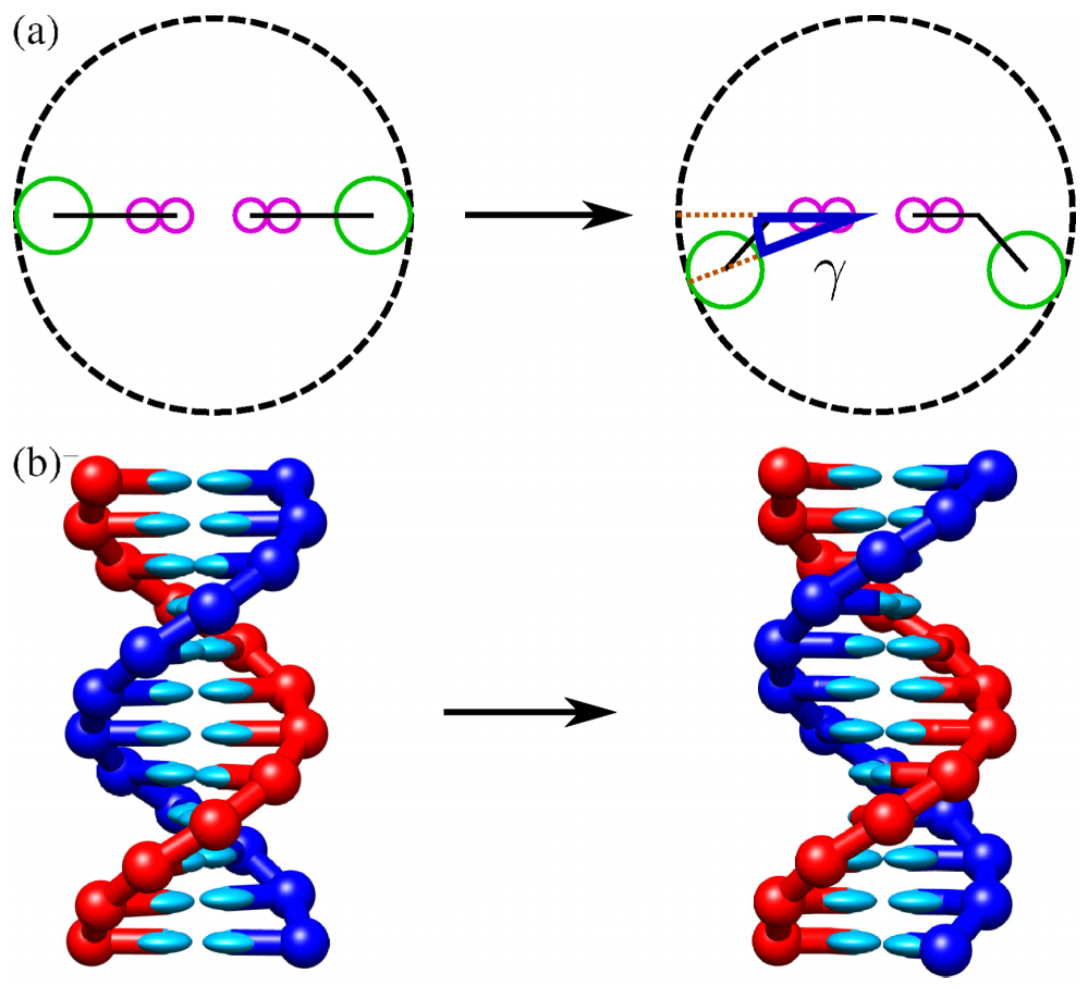
\includegraphics[width=0.85\textwidth]{oxdna_oxdna2.png}\\
\end{center}
\textit{(a) oxDNA1 and oxDNA2 nucleotides: the base vector $\bm{b}$ is horizontally oriented from left to right, whereas the base normal $\bm{n}$ points away from the observer.}\\[3pt]
\textit{(b) The angled backbone interaction sites leads to the correct geometry with major and minor grooves.} 
\end{column}
\end{columns}

\end{frame}

\begin{frame}
\frametitle{Angles and Vectors}

\begin{columns}
\begin{column}{0.56\textwidth}
\textbf{Relative distance vectors} are defined between two nucleotides $i$ and $j$
\begin{itemize}
\setlength\itemsep{3pt}
\item backbone interaction sites\\
$\bm{r}_{back, ij}=\bm{r}_{back,i} - \bm{r}_{back,j}$
\item stacking interaction sites\\
$\bm{r}_{stack, ij}=\bm{r}_{stack,i} - \bm{r}_{stack,j}$
\item hydrogen-bonding interaction sites\\
$\bm{r}_{base, ij}=\bm{r}_{base,i} - \bm{r}_{base,j}$
\item mixed sites\\
$\bm{r}_{back-base, ij}=\bm{r}_{back,i} - \bm{r}_{base,j}$
$\bm{r}_{base-back, ij}=\bm{r}_{base,i} - \bm{r}_{back,j}$
\end{itemize}
\textbf{Relative angles} are defined using the above vectors, the base vector $\bm{b}$ and base normal $\bm{n}$ 
\vspace*{0.25cm}
\begin{itemize}
\item[] $\cos(\theta_1) = -\,\hat{\bm{b}}_i \cdot \hat{\bm{b}}_j$
\item[] $\cos(\theta_2) = -\,\hat{\bm{b}}_i \cdot \hat{\bm{r}}_{base, ij}$
\item[] $\cos(\theta_3) = \hat{\bm{b}}_j \cdot \hat{\bm{r}}_{base, ij}$
\item[] $\qquad\vdots\qquad\vdots\qquad\vdots$
\end{itemize}
\end{column}

\begin{column}{0.44\textwidth}
\vspace*{-0.25cm}
\begin{center}
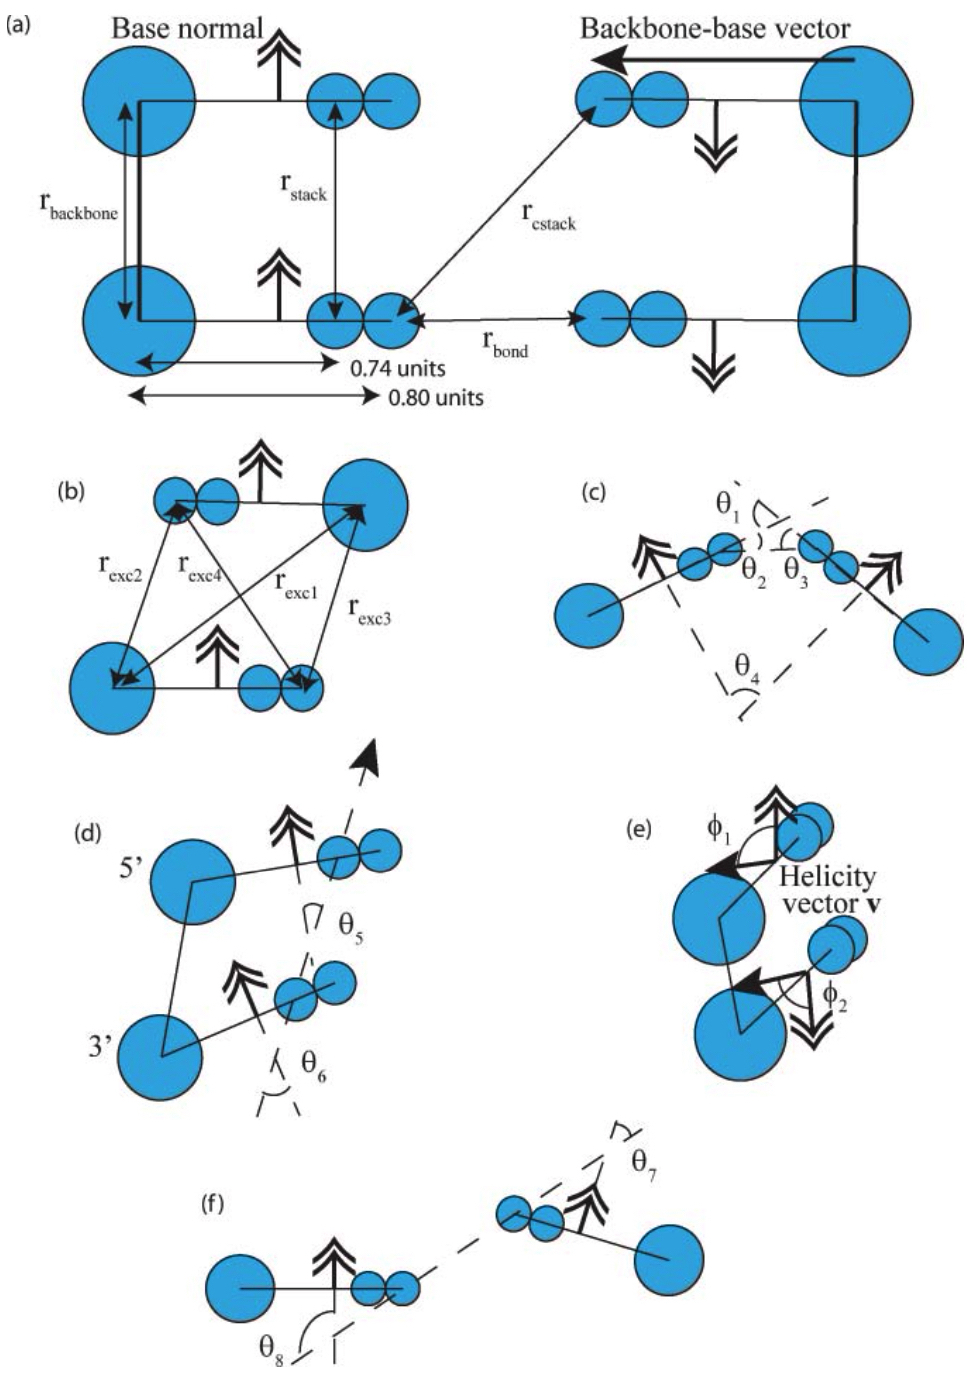
\includegraphics[width=0.9\textwidth]{oxdna.jpg}
\textit{oxDNA1 vectors and angles}
\end{center}
\end{column}
\end{columns}

\end{frame}

\begin{frame}
\frametitle{Potential Forms}
\textbf{Elementary potentials} are used, which take distances or angles as arguments.\\[10pt]
\begin{itemize}
\setlength\itemsep{7pt}
\item FENE springs for backbone connectivity\\
$V_{FENE}(r,\epsilon,r^0,\Delta)=-\frac{\epsilon}{2}\ln\left(1-\frac{(r-r^0)^2}{\Delta^2}\right)$
\item Morse potential for stacking and hydrogen-bonding\\
$V_{Morse}(r,\epsilon,r^0,a)=\epsilon(1-\exp(-a(r-r^0)))^2$
\item Harmonic potential for cross-stacking and coaxial stacking\\
$V_{harm}(r,k,r^0)=\frac{k}{2}(r-r^0)^2$
\item Lennard-Jones potential for excluded volume\\
$V_{LJ}(r,\epsilon,\sigma)=4\epsilon\left(\left(\frac{\sigma}{r}\right)^{12} - \left(\frac{\sigma}{r}\right)^6\right)$
\item Quadratic terms for angular modulations\\
$V_{mod}(\theta,a,\theta^0)=1-a(\theta-\theta^0)^2$
\item Quadratic smoothing terms for truncation\\
$V_{smooth}(x,b,x^c)=b(x-x^c)^2$
\item Debye-H\"uckel potential for elextrostatics\\
$V_{DH}(r, \lambda)=\frac{q_{eff}}{4\pi\epsilon_0\epsilon_r} \exp(-r/\lambda)/r$
\end{itemize}

\end{frame}

\begin{frame}
\frametitle{Modulation Factors}
The above potentials are used directly or in angular and radial modulation factors $f_{1,\dots,6}$.
\scriptsize
\begin{flalign*}
  &f_{1}(r) = 
   \begin{cases}
  V_{Morse}(r, \epsilon, r^{0}, a) &\mbox{if } r^{low} < r < r^{high}, \\
  \epsilon V_{smooth}(r, b^{low}, r^{c,low}) &\mbox{if } r^{c, low} < r < r^{low}, \\
  \epsilon V_{smooth}(r, b^{high}, r^{c,high}) &\mbox{if } r^{high} < r < r^{c, high}, \\
  0 &\mbox{otherwise}
  \end{cases}\\
  &f_{2}(r) = 
  \begin{cases}
  V_{harm}(r, k, r^{0})-V_{harm}(r^{c}, k, r^{0}) &\mbox{if } r^{low} < r , r^{high}, \\
  kV_{smooth}(r , b^{low}, r^{c,low}) &\mbox{if } r^{c, low} < r < r^{low}, \\
  kV_{smooth}(r , b^{high}, r^{c,high}) &\mbox{if } r^{high} < r < r^{c, high}, \\
  0 &\mbox{otherwise}
  \end{cases}\\
  &f_{3}(r) = 
  \begin{cases}
  V_{LJ}(r, \epsilon, \sigma) &\mbox{if } r < r^{\star}, \\
  \epsilon V_{smooth}(r, b, r^{c}) &\mbox{if } r^{\star} < r < r^{c}, \\
  0 &\mbox{otherwise}
  \end{cases}\\
  &f_{4}(\theta) = 
  \begin{cases}
  V_{mod}(\theta, a, \theta^{0}) &\mbox{if } \theta^{0} - \Delta\theta^{\star} < \theta < \theta^{0} + \Delta\theta^{\star}, \\
  V_{smooth}(\theta, b, \theta^{0} - \Delta\theta^{c}) &\mbox{if } \theta^{0} - \Delta\theta^{c} < \theta < \theta^{0} - \Delta\theta^{\star}, \\
  V_{smooth}(\theta, b, \theta^{0} + \Delta\theta^{c}) &\mbox{if } \theta^{0} + \Delta\theta^{\star} < \theta < \theta^{0} + \Delta\theta^{c}, \\
  0 &\mbox{otherwise}
  \end{cases}\\
  &f_{5}(x) = 
  \begin{cases}
  1 &\mbox{if } x > 0, \\
  V_{mod}(x,a,0) &\mbox{if } x^{\star} < x < 0, \\
  V_{smooth}(x, b, x^c) &\mbox{if } x^{c} < x< x^{\star}, \\
  0 &\mbox{otherwise}
  \end{cases}\\
  &f_{6}(\theta) = 
  \begin{cases}
  V_{smooth}(\theta, b, \theta^c) &\mbox{if } \theta\ge\theta^{c}, \\
  0 &\mbox{otherwise}
  \end{cases}\\
\end{flalign*}

\end{frame}

\begin{frame}
\frametitle{Interactions}
The \textbf{oxDNA2 potential} consists of \textbf{1 bonded} and \textbf{6 pair interactions}.
\vspace*{0.25cm}
\begin{itemize}
\setlength\itemsep{5pt}
\small
\item \textbf{Backbone connectivity} (bonded): $V_{backbone} = V_{FENE}(.)$
\item \textbf{Excluded volume} (pair)\\
$V_{excv} = f_3(r_{back-back}, ..)+f_3(r_{back-base}, ..)+f_3(r_{base-back}, ..)+f_3(r_{base-base}, ..)$
\item \textbf{Stacking} (pair): $V_{stack} = f_1(\cdot)\times f_4(\cdot)\times f_4(\cdot)\times f_4(\cdot)\times f_5(\cdot)\times f_5(\cdot)$
\item \textbf{Hydrogen-bonding} (pair): $V_{HB} = f_1(\cdot)\times f_4(\cdot)\times f_4(\cdot)\times f_4(\cdot)\times f_4(\cdot)\times f_4(\cdot)$
\item \textbf{Cross-stacking} (pair)\\
$V_{x-stack} = f_2(\cdot)\times f_4(\cdot)\times f_4(\cdot)\times f_4(\cdot)\times\Big\{f_4(\cdot)+ f_4(\cdot)\Big\} \times \Big\{f_4(\cdot)+ f_4(\cdot)\Big\} \times\Big\{f_4(\cdot)+ f_4(\cdot)\Big\}$
\item \textbf{Coaxial stacking} (pair)\\
$V_{coaxial-stack} = f_2(\cdot)\times f_4(\cdot)\times \times\Big\{f_4(\cdot)+ f_6(\cdot)\Big\} \times \Big\{f_4(\cdot)+ f_4(\cdot)\Big\} \times\Big\{f_4(\cdot)+ f_4(\cdot)\Big\}$
\item \textbf{Electrostatic} (pair): $V_{elec} = V_{DH}(\cdot)$
\end{itemize}

\vspace*{0.25cm}
The complete potential contains sums over consecutive nucleotides on the same strand and all other pairs.
\begin{flalign*}
V = &\sum_{nearest\ neighbours}(V_{backbone} + V'_{excv} + V_{stack}) \\ 
+ &\sum_{other\ pairs}(V_{elec} + V_{HB} + V_{x-stack} + V_{coaxial-stack} + V_{elec})
\end{flalign*}

\end{frame}


\begin{frame}
\frametitle{Summary}
\vspace*{0.25cm}
\small
\begin{itemize}
\setlength\itemsep{5pt}
\item The oxDNA model uses a \textbf{top-down coarse-graining approach} with rather complex \textbf{bespoke interactions}.
\item The oxDNA potential comprises \textbf{one bonded interaction} and \textbf{six pair interactions}. As strands denature, there is no residual memory of other conformations as is often the case with 3+body interactions.
\item The \textbf{thermodynamic properties} of oxDNA are basically those of the \textbf{SantaLucia nearest-neighbour model}, thought to be an \textbf{exact empirical fit} experiments. 
\item \textbf{Uniquely among coarse-grained  models} at this level of detail, oxDNA is able to describe the \textbf{thermodynamics of duplex formation} and provide an \textbf{accurate average representation} of the structure and mechanics of \textbf{both single-stranded and double stranded DNA and its assemblies}.
\item oxDNA2 features \textbf{sequence-specific hydrogen-bonding and stacking interaction strengths}. But there is \textbf{no intrinsic sequence-specific curvature or elasticity} ($\Rightarrow$ oxDNA3).  
\end{itemize}
\vspace*{0.25cm}
[1] T. Ouldridge, A. Louis, and J. Doye, \href{https://doi.org/10.1063/1.3552946}{Structural, Mechanical, and Thermodynamic Properties of a Coarse-Grained DNA Model}, \textit{J. Chem. Phys.} \textbf{134}, 085101 (2011).\\[7pt]
[2] B. Snodin, et al., \href{https://doi.org/10.1063/1.4921957}{Introducing Improved Structural Properties and Salt Dependence into a Coarse-Grained Model of DNA}, \textit{J. Chem. Phys.}  \textbf{142}, 234901 (2015).

\end{frame}


\section{oxDNA Software}

\begin{frame}
\frametitle{Overview}

We will use the following software\\[10pt]

\begin{itemize}
\setlength\itemsep{10pt}
\item LAMMPS version of oxDNA\\
The implementation of oxDNA1, oxDNA2 and oxRNA2 in the LAMMPS code via the \texttt{CG-DNA USER} package 
\item Standalone version of oxDNA\\
The original re-implementation of oxDNA1, which was extended to oxDNA2 and oxRNA2
\item tacoxDNA\\
A suite of tools and converters
\item oxView\\
A visualisation and data manipulation toolkit
\end{itemize}

\end{frame}

\begin{frame}
\frametitle{LAMMPS Version}
\begin{itemize}
\item \textbf{L}arge-scale \textbf{A}tomic/\textbf{M}olecular \textbf{M}assively \textbf{P}arallel \textbf{S}imulator
\item Available from the LAMMPS website at \href{https://www.lammps.org}{https://www.lammps.org}\\
Distributed under GPL v2 by Sandia National Laboratories\\
Latest stable release 23rd June 2022 (initial release 1995)
\item Popular
\begin{itemize}
\item 405,000 downloads between September 2004 and June 2021
\item 1,400 forks on GitHub, ca. 100 direct contributors
\end{itemize}
\item \textbf{Versatile}
\begin{itemize}
\item Very \textbf{advanced molecular dynamics capabilities}
\item Code distributed over \textbf{91 standard and \texttt{USER} packages}
\item Supported on \textbf{CPU-, multicore- and GPU-architectures}, but not all packages offer all options
\item REPLICA: collection of multi-replica methods, e.g. parallel tempering
\item PLUMED: free energy library, enhanced sampling
\item COLVARS: collective variables library, advanced sampling methods like metadynamics, umbrella sampling, adaptive biasing force 
\end{itemize}
\item \textbf{Extendable}
\begin{itemize}
\item Object-oriented C++ class structure
\item Top-level classes that are visible everywhere in the code
\item Virtual parent classes derived from top-level classes
\item Extensive use of polymorphism
\end{itemize}
\end{itemize}


\end{frame}

\begin{frame}[fragile]
\frametitle{LAMMPS Version}
\small 
Building the LAMMPS version with standard make
\begin{itemize}
\item Requires C/C++ compiler that supports the C++11 standard
\item Change to \texttt{/src} in your LAMMPS directory
\item Load \texttt{ASPHERE}, \texttt{MOLECULE} and \texttt{\textcolor{red}{CG-DNA}} packages (minimal requirement)\\
\linespread{0.4}
\begin{lstlisting}
make yes-asphere yes-molecule yes-cg-dna
\end{lstlisting}
\item Check modules are loaded and clean

\begin{lstlisting}
make ps

Installed YES: package ASPHERE
Installed YES: package CG-DNA
Installed YES: package MOLECULE
\end{lstlisting}

\item Compile the serial and/or parallel version using the default \texttt{Makefiles} in \texttt{/src/MAKE}
\begin{lstlisting}
make [-j4] serial
make [-j4] mpi
\end{lstlisting}
\item More \texttt{Makefile} configurations are in \texttt{/src/MAKE/MACHINES}
\end{itemize}
\linespread{1.0}\vspace*{0.25cm}
[3] O. Henrich, Y. A. Guti\'errez Fosado, T. Curk, and T. E. Ouldridge, \href{https://doi.org/10.1140/epje/i2018-11669-8}{Coarse-Grained Simulation of DNA Using LAMMPS: An Implementation of the OxDNA Model and Its Applications}, \textit{Eur. Phys. J. E} \textbf{41}, (2018).\\[3pt]
[4] LAMMPS CG-DNA Documentation \href{https://docs.lammps.org/PDF/CG-DNA.pdf}{https://docs.lammps.org/PDF/CG-DNA.pdf}
\end{frame}

\begin{frame}
\frametitle{Standalone Version}

\begin{itemize}
\setlength\itemsep{10pt}
\item \textbf{oxDNA} code includes oxDNA1, oxDNA2 and oxRNA 
\item Available from \href{https://github.com/lorenzo-rovigatti/oxDNA}{https://github.com/lorenzo-rovigatti/oxDNA}\\
Distributed under GPL v3\\
Latest stable release 3.4.2 (8th Sept 2022)
\item 11 forks on GitHub, half a dozen contributors
\item Very \textbf{advanced Monte Carlo capabilities} like \textbf{Virtual-Move Monte Carlo} (VMMC) 
\item Supported on \textbf{single-core CPU- and single GPU-architectures}
\item Very extensive suite of \textbf{oxDNA Analysis Tools (OAT)} of bespoke postprocessing and analysis scripts 
\end{itemize}

\end{frame}

\begin{frame}[fragile]
\frametitle{Standalone Version}
Building the serial standalone version for CPU-architectures with standard CMake

\begin{itemize}
\item Requires

\begin{itemize}
\item C/C++ compiler that supports the C++14 standard
\item CMake version $\ge 3.5$
\item optionally CUDA toolkit version $\ge 10$
\end{itemize}
\item Change to the oxDNA top-level directory
\linespread{0.4}
\begin{lstlisting}
cd oxDNA
\end{lstlisting}
\item Create a build directory and change to it
\begin{lstlisting}
mkdir build
cd build
\end{lstlisting}
\item Create Makefiles, specify additonal options
\begin{lstlisting}
cmake ..
\end{lstlisting}
\item Compile the serial version
\begin{lstlisting}
make [-j4]
\end{lstlisting}
\end{itemize}

[5] oxDNA Documentation \href{https://lorenzo-rovigatti.github.io/oxDNA}{https://lorenzo-rovigatti.github.io/oxDNA}\\[3pt]
[6] oxDNA Website \href{https://dna.physics.ox.ac.uk}{https://dna.physics.ox.ac.uk}

\end{frame}

\begin{frame}
\frametitle{tacoxDNA Tools and Converters}

Available
\begin{itemize}
\item as webserver at \href{http://tacoxdna.sissa.it}{http://tacoxdna.sissa.it}
\item as standalone Python code from \href{https://github.com/lorenzo-rovigatti/tacoxDNA}{https://github.com/lorenzo-rovigatti/tacoxDNA}
\end{itemize}

\vspace*{0.5cm}
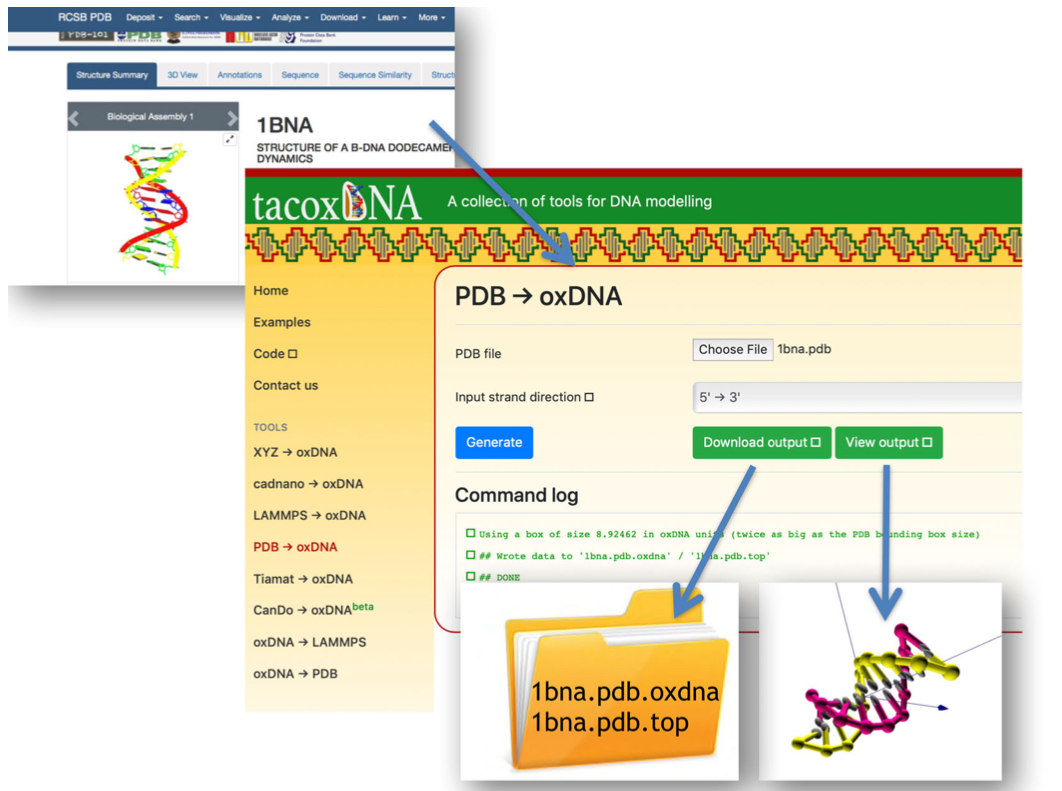
\includegraphics[width=0.45\textwidth]{tacoxDNA_pdb.jpg}
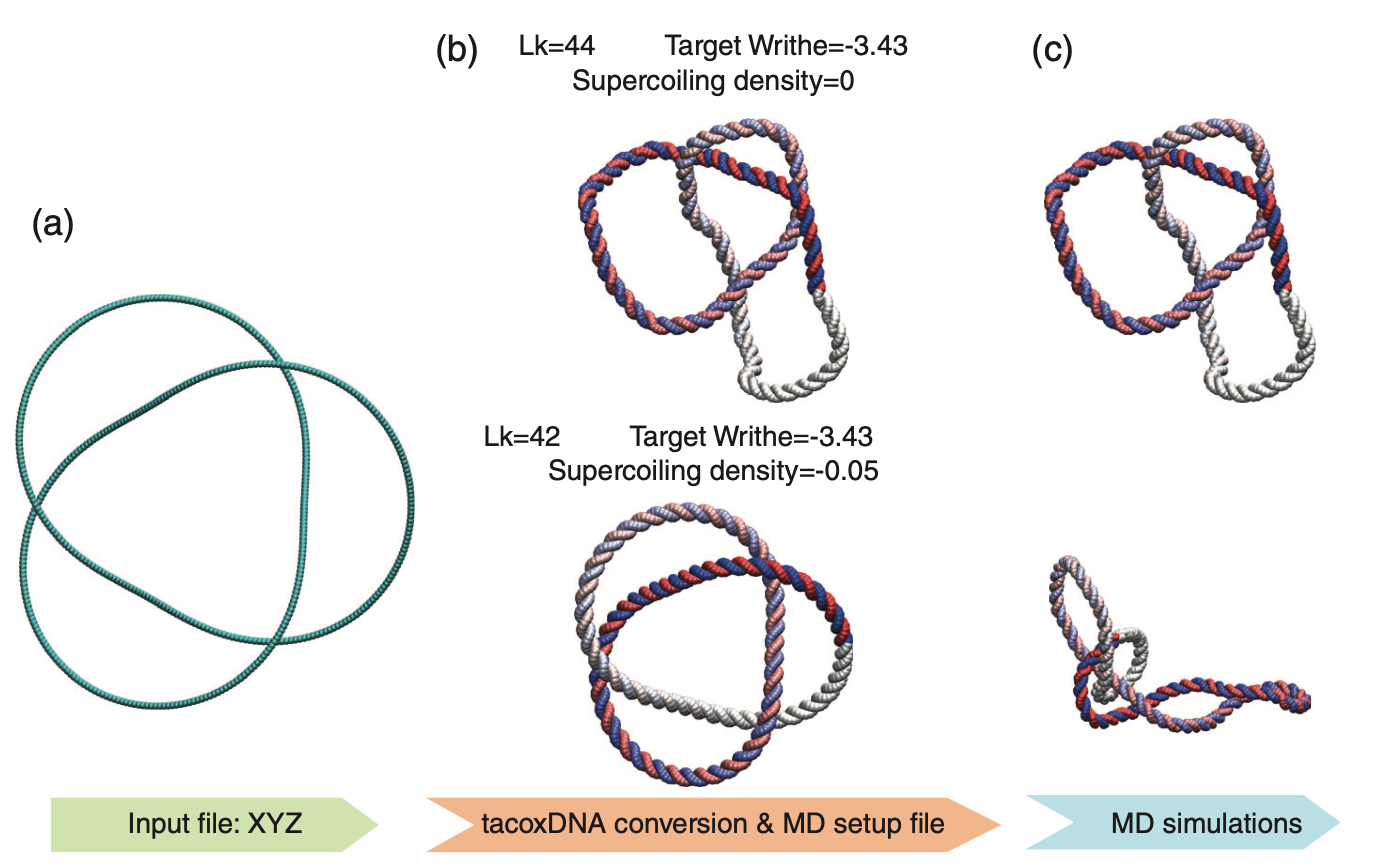
\includegraphics[width=0.45\textwidth]{tacoxDNA_trefoil.jpg}\\
\vspace*{0.5cm}

[7] A. Suma, et al., \href{https://doi.org/10.1002/jcc.26029}{TacoxDNA: A User-Friendly Web Server for Simulations of Complex DNA Structures, from Single Strands to Origami}, \textit{J. Comput. Chem.} \textbf{40}, 2586 (2019).

\end{frame}
\begin{frame}

\frametitle{tacoxDNA Tools and Converters}

\begin{columns}
\begin{column}{0.55\textwidth}
\vspace*{0.25cm}\\
A variety of format conversions is supported. The native oxDNA format can also be used as intermediate.
\vspace*{0.25cm}
\begin{itemize}
\setlength\itemsep{7pt}
\item LAMMPS format $\Leftrightarrow$ native oxDNA format
\item PDB format $\Leftrightarrow$ native oxDNA format
\item XYZ format $\Rightarrow$ native oxDNA format
\item cadnano $\Rightarrow$ native oxDNA format
\item CanDo $\Rightarrow$ native oxDNA format
\item Tiamat $\Rightarrow$ native oxDNA format
\end{itemize}
\end{column}

\begin{column}{0.45\textwidth}
\begin{center}
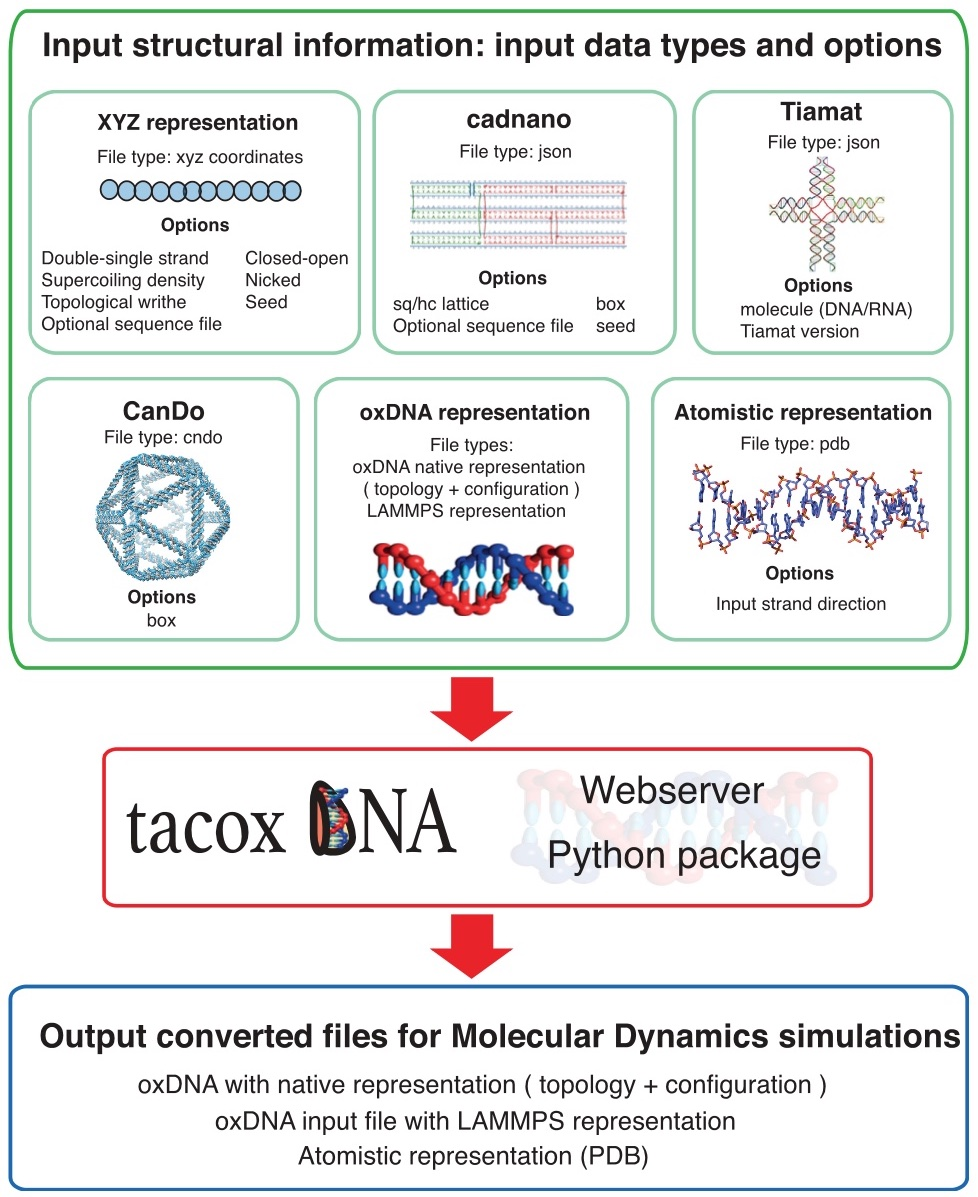
\includegraphics[width=0.90\textwidth]{tacoxDNA_schematic.jpg}
\end{center}
\end{column}
\end{columns}
\vspace*{0.25cm}
[7] A. Suma, et al., \href{https://doi.org/10.1002/jcc.26029}{TacoxDNA: A User-Friendly Web Server for Simulations of Complex DNA Structures, from Single Strands to Origami}, \textit{J. Comput. Chem.} \textbf{40}, 2586 (2019).

\end{frame}

\begin{frame}[fragile]
\frametitle{oxView Visualisation and Manipulation Toolkit}
\small

\begin{columns}

\begin{column}{0.6\textwidth}
\textbf{oxView} is a webbrowser-based visualiser
\begin{itemize}
\item Can load structures with over 1 million nucleotides
\item Create videos from simulation trajectories
\item Allow users to perform basic edits to DNA and RNA designs
\end{itemize}
\vspace*{0.25cm}
Available from \href{https://github.com/sulcgroup/oxdna-viewer}{https://github.com/sulcgroup/oxdna-viewer}
\begin{itemize}
\item Navigate down to the \texttt{README.md} and click \href{https://sulcgroup.github.io/oxdna-viewer}{Try it!}\\or
\item Load \href{https://sulcgroup.github.io/oxdna-viewer}{https://sulcgroup.github.io/oxdna-viewer}\\or
\item Run locally on \texttt{localhost:8000} by starting a python server in your oxView directory
\begin{lstlisting}
python -m http.server 8000
\end{lstlisting}
\end{itemize}

\end{column}
\begin{column}{0.4\textwidth}
\begin{center}
\vspace*{-0.25cm}
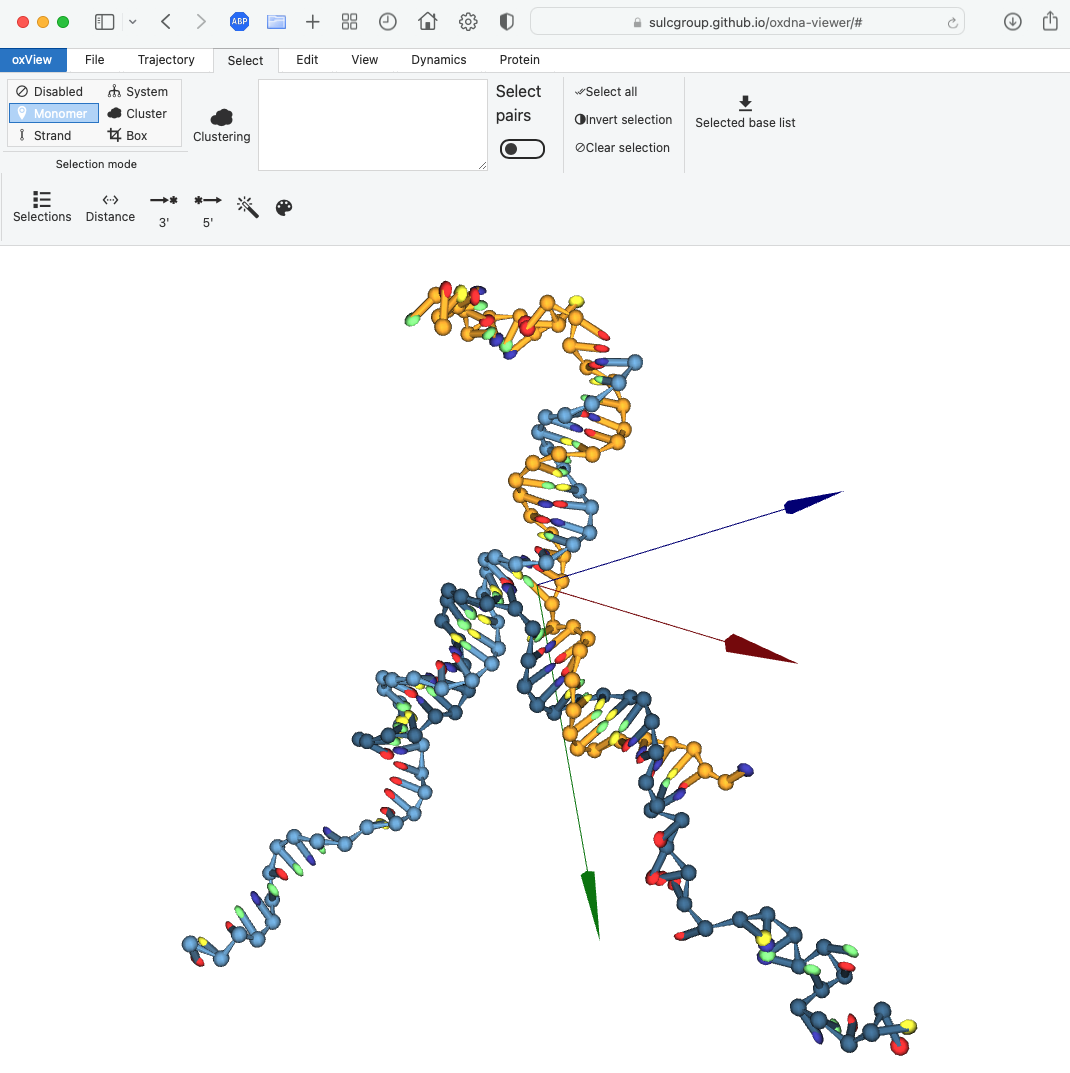
\includegraphics[width=\textwidth]{oxviewer.png}
\end{center}
\end{column}
\end{columns}

\vspace*{0.25cm}

[8] E. Poppleton, et al., \href{https://doi.org/10.1093/nar/gkaa417}{Design, Optimization and Analysis of Large DNA and RNA Nanostructures through Interactive Visualization, Editing and Molecular Simulation}, \textit{Nucleic Acids Res.} \textbf{48}, e72 (2020).\\[3pt]

[9] J. Bohlin, et al., \href{https://doi.org/10.1038/s41596-022-00688-5}{Design and Simulation of DNA, RNA and Hybrid Protein–Nucleic Acid Nanostructures with OxView}, \textit{Nat. Protoc.} \textbf{17}, 1762 (2022).


\end{frame}

\section{Practical Exercises}
\small

\begin{frame}[fragile]
\frametitle{(I) Creating an Initial Configuration}

\begin{itemize}
\item Clone the oxDNA tutorial directory from GitHub
\begin{lstlisting}
git clone https://github.com/ohenrich/oxDNA_tutorial.git 
\end{lstlisting}

\item Navigate to the first exercise
\begin{lstlisting}
cd exercises/1_initial_config
\end{lstlisting}

\item Inspect the file \texttt{sequence.txt}
\begin{lstlisting}
vi sequence.txt
DOUBLE AAAAAACGCGAAA...
\end{lstlisting}
The keyword \texttt{DOUBLE} indicates that we will create double-stranded DNA. Omitting the keyword produces a single-stranded configuration.

\item Check syntax of configuration generator
\linespread{0.4}
\begin{lstlisting}
python generate-sa.py

Usage: generate-sa.py <box size> <file with sequences>
\end{lstlisting}

\item Generate an initial configuration in a box size 100
\begin{lstlisting}
python generate-sa.py 100 sequence.txt

Found duplex of 63 bases
nstrands, nnucl =  2 126
Adding duplex of 63 bases
done line 1 / 1, now at 126/126
ALL DONE. just generated 'generated.dat' and 'generated.top'
\end{lstlisting}
\end{itemize}

\end{frame}

\begin{frame}[fragile]
\frametitle{(I) Creating an Initial Configuration}

\begin{itemize}
\item Inspect the oxDNA standalone format: topology file
\linespread{0.4}
\begin{lstlisting}
vi generated.top

126 2             # total no. of nucleotides and strands
1 A -1 1          # strand ID, nucleotide type, 3' partner, 5' partner
1 A 0 2
1 A 1 3
1 A 2 4
...
\end{lstlisting}


\item Inspect the oxDNA standalone format: configuration file
\begin{lstlisting}
vi generated.dat

t = 0                           # timestep
b = 100.0 100.0 100.0           # box dimensions
E = 0. 0. 0.                    # energy 
81.10076700045578 45.544279111797685 26.695973276367443 0.6836324286755338 0.6187606869041726 -0.3870166854349663 0.4842717557006389 0.012139188631672909 0.8748334165599674 0.0 0.0 0.0 0.0 0.0 0.0
81.55953447082155 45.3431814998625 26.89033700942101 0.233605215000666 0.9618090481628894 -0.1426602901878769 0.4842717557006389 0.012139188631672909 0.8748334165599674 0.0 0.0 0.0 0.0 0.0 0.0
...

# position, base vector, base normal, velocity, angular momentum
\end{lstlisting}

\item Rename the files
\begin{lstlisting}
mv generated.top dsDNA_init.top
mv generated.dat dsDNA_init.dat
\end{lstlisting}

\end{itemize}

\end{frame}

\begin{frame}[fragile]
\frametitle{(I) Creating an Initial Configuration}
\normalsize
\begin{itemize}
\item Download the topology and configuration files to your local host in a working directory
\begin{lstlisting}
scp username@hostname:/path/to/oxDNA_tutorial/
                                exercises/1_initial_config/dsDNA_init* .
\end{lstlisting}
\end{itemize}

\begin{columns}

\begin{column}{0.48\textwidth}

\begin{itemize}
\setlength\itemsep{15pt}
\item Open oxView in your browser,\\
click on the 'Open' tab,\\
navigate to your local working directory and load the two files

\item Inspect and edit the visualisation, e.g. by rotating and translating the dsDNA molecule
\end{itemize}
\end{column}

\begin{column}{0.48\textwidth}

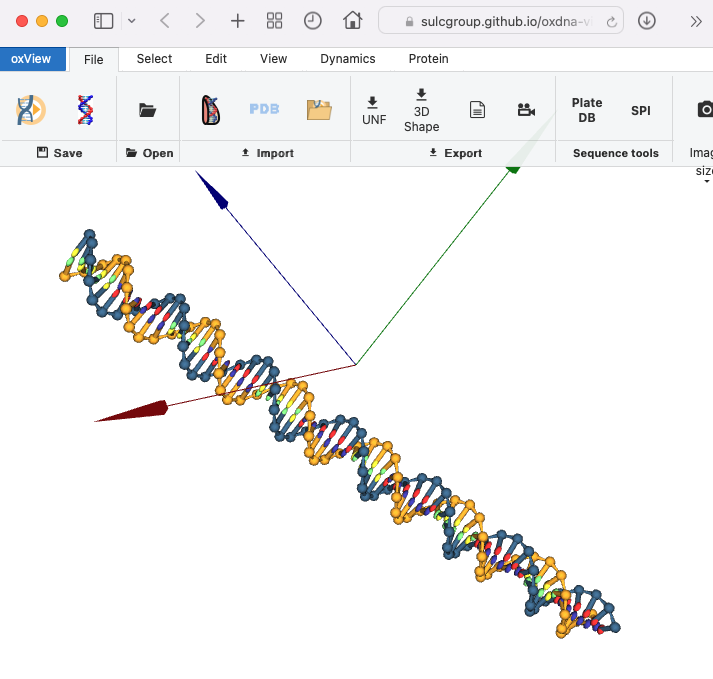
\includegraphics[width=\textwidth]{oxView_dsDNA_init.png}

\end{column}
\end{columns}

\end{frame}

\begin{frame}[fragile]
\frametitle{(II) Equilibration Using The Standalone Code}

\begin{itemize}
\item 
\begin{lstlisting}

\end{lstlisting}
\end{itemize}

\end{frame}

\begin{frame}[fragile]
\frametitle{(II) Equilibration Using The Standalone Code}

\begin{itemize}
\item 
\begin{lstlisting}

\end{lstlisting}
\end{itemize}

\end{frame}

\begin{frame}[fragile]
\frametitle{}

\begin{itemize}
\item 
\begin{lstlisting}

\end{lstlisting}
\end{itemize}

\end{frame}

\begin{frame}[fragile]
\frametitle{}

\begin{itemize}
\item 
\begin{lstlisting}

\end{lstlisting}
\end{itemize}

\end{frame}

\begin{frame}[fragile]
\frametitle{}

\begin{itemize}
\item 
\begin{lstlisting}

\end{lstlisting}
\end{itemize}

\end{frame}

\end{document}
